\documentclass[titlepage, 12pt]{article}
\usepackage[utf8]{inputenc}
\usepackage[spanish]{babel}
\usepackage[margin=3cm]{geometry}
\usepackage{graphicx}
\usepackage{xcolor}
\usepackage{blindtext}
\usepackage{hyperref}

\begin{document}

\begin{titlepage}
	\centering
	{\scshape\LARGE Escuela Superior de Cómputo. \par}
	\vspace{1cm}
	
	\includegraphics[width=0.4\textwidth]{escom.png}\par\vspace{1cm}
	
	{\scshape\Large Web Application Development.\par}
	\vspace{1cm}
	
	{\Large\bfseries ``Práctica 1: Servlets "\par}
	\vspace{1cm}
	
    {\Large\itshape Integrantes:  \\ Guadarrama Ascencio Juan Carlos. \\ Ornelas García Luis Ángel. \\ Sampayo Hernández Mauro. \par}
	\vspace{1cm}
	
	\vfill
	Profesor:\par
	Enrique Zarate M. en C. José Asunción.
	\vfill
\end{titlepage}

\tableofcontents
\newpage

\listoffigures
\newpage

\pagenumbering {arabic}

\section{Introducción:}

Los servlets son modulos java que nos sirven para extender las capacidades de los servidores web. Aunque es una definición un poco ambigua los servlets son programas para los servidores, mientras que los applets son programas para los clientes y los middlets son programas para microdispositivos. Dentro de una evolución cronologica los servlets son la siguiente etapa de los CGI. En algunas bibliografias son referenciados como CGI de 2ª generación, la cual comparten con lenguajes como ASP, PHP y JSP (que al fin y al cabo son servlets). El uso de los servlets viene a ser en un tanto por ciento elevando el del desarrollo de páginas web dinámicas (en contenido y diseño) apoyándose además en la potencia que nos proporciona el lenguaje Java. \par\vspace{0.5cm}

Podremos desarrollar desde un simple servlet que nos muestre una página web simple saludandonos hasta uno que se conecte a una base de datos utilizando un pool de conexiones, encriptando la información en su envio, accediendo a bases de datos distribuidas y manteniendo su información de forma persistente en un EJB. Todo ello para conseguir una información dinámica. A partir de aqui las posibilidades son “infinitas”.

\pagebreak

\section{Conceptos:}

\subsection{Servlets}
Son la tecnología de la plataforma Java para ampliar y mejorar los servidores web. Los servlets proporcionan un método basado en componentes e independiente de la plataforma para crear aplicaciones basadas en la Web, sin las limitaciones de rendimiento de los programas CGI. Y a diferencia de los mecanismos de extensión de servidores propietarios (como la API del servidor Netscape o los módulos Apache), los servlets son independientes del servidor y de la plataforma. Esto le permite seleccionar la mejor estrategia para sus servidores, plataformas y herramientas.\par\vspace{0.5cm}

\subsection{Conectores}
 Los conectores TCP/IP en concreto, se utilizan para implementar conexiones basadas en flujo, punto a punto, bidireccionales y fiables entre nodos de Internet. Se puede utilizar un conector para conectar el sistema de E/S de Java a otros programas que pueden residir en la máquina local o en cualquier otra máquina de Internet. \par\vspace{0.5cm}
 
\subsection{JDBC (Java Database Connectivity)}
Es el estándar del sector para la conectividad independiente de las bases de datos entre el lenguaje de programación Java y una amplia gama de bases de datos SQL y otras fuentes de datos tabulares, como hojas de cálculo o archivos planos. La API JDBC proporciona una API de nivel de llamada para el acceso a bases de datos basadas en SQL.

La tecnología JDBC permite utilizar el lenguaje de programación Java para explotar las capacidades de "escribir una vez y ejecutar en cualquier lugar" para las aplicaciones que requieren acceso a los datos de la empresa. Con un controlador compatible con la tecnología JDBC, podrá conectar todos los datos de la empresa incluso en un entorno heterogéneo.

\pagebreak

\section{Desarrollo:}

A continuación se muestran capturas de la aplicación web:

\subsection{Inicio}
    \begin{figure}[h]
        \caption{Inicio.}
        \centering
        \includegraphics[width=0.8\textwidth]{capturasProyectoBase/index.PNG} \par\vspace{0.5cm}
    \end{figure}

\subsection{Tabla de Multiplicar}   
    \begin{figure}[h]
        \caption{Tabla de Multiplicar.}
        \centering
        \includegraphics[width=0.8\textwidth]{capturasProyectoBase/tablaMultiplicar.PNG} \par\vspace{0.5cm}
    \end{figure}
    
    \clearpage

\subsection{CRUD Categorías}
    \begin{figure}[h]
        \caption{CRUD Categorías (Mostrar Categorías).}
        \centering
        \includegraphics[width=0.8\textwidth]{capturasProyectoBase/mostrarCategorias.PNG} \par\vspace{0.5cm}
    \end{figure}
    
    \begin{figure}[h]
        \caption{CRUD Categorías (Crear Categoría 01).}
        \centering
        \includegraphics[width=0.8\textwidth]{capturasProyectoBase/crearCategoria1.PNG} \par\vspace{0.5cm}
    \end{figure}
    
    \clearpage
    
    \begin{figure}[h]
        \caption{CRUD Categorías (Crear Categoría 02).}
        \centering
        \includegraphics[width=0.8\textwidth]{capturasProyectoBase/crearCategoria2.PNG} \par\vspace{0.5cm}
    \end{figure}
    
    \begin{figure}[h]
        \caption{CRUD Categorías (Crear Categoría 03).}
        \centering
        \includegraphics[width=0.8\textwidth]{capturasProyectoBase/crearCategoria3.PNG} \par\vspace{0.5cm}
    \end{figure}
    
    \clearpage
    
     \begin{figure}[h]
        \caption{CRUD Categorías (Ver Categoría).}
        \centering
        \includegraphics[width=0.8\textwidth]{capturasProyectoBase/verCategoria.PNG} \par\vspace{0.5cm}
    \end{figure}
    
     \begin{figure}[h]
        \caption{CRUD Categorías (Actualizar Categoría 01).}
        \centering
        \includegraphics[width=0.8\textwidth]{capturasProyectoBase/actualizarCategoria1.PNG} \par\vspace{0.5cm}
    \end{figure}
    
    \clearpage
    
    \begin{figure}[h]
        \caption{CRUD Categorías (Actualizar Categoría 02).}
        \centering
        \includegraphics[width=0.8\textwidth]{capturasProyectoBase/actualizarCategoria2.PNG} \par\vspace{0.5cm}
    \end{figure}
    
    \begin{figure}[h]
        \caption{CRUD Categorías (Actualizar Categoría 03).}
        \centering
        \includegraphics[width=0.8\textwidth]{capturasProyectoBase/actualizarCategoria3.PNG} \par\vspace{0.5cm}
    \end{figure}
    
    \clearpage
    
    \begin{figure}[h]
        \caption{CRUD Categorías (Actualizar Categoría 04).}
        \centering
        \includegraphics[width=0.8\textwidth]{capturasProyectoBase/actualizarCategoria4.PNG} \par\vspace{0.5cm}
    \end{figure}
    
    \begin{figure}[h]
        \caption{CRUD Categorías (Eliminar Categoría 01).}
        \centering
        \includegraphics[width=0.8\textwidth]{capturasProyectoBase/eliminarCategoria1.PNG} \par\vspace{0.5cm}
    \end{figure}
    
    \clearpage
    
    \begin{figure}[h]
        \caption{CRUD Categorías (Eliminar Categoría 02).}
        \centering
        \includegraphics[width=0.8\textwidth]{capturasProyectoBase/eliminarCategoria2.PNG} \par\vspace{0.5cm}
    \end{figure}

\subsection{CRUD Productos}
    \begin{figure}[h]
        \caption{CRUD Productos (Mostrar Productos).}
        \centering
        \includegraphics[width=0.8\textwidth]{capturasProyectoBase/mostrarProductos.PNG} \par\vspace{0.5cm}
    \end{figure}
    
    \clearpage
    
    \begin{figure}[h]
        \caption{CRUD Productos (Crear Producto 01).}
        \centering
        \includegraphics[width=0.8\textwidth]{capturasProyectoBase/crearProducto1.PNG} \par\vspace{0.5cm}
    \end{figure}
    
    
     \begin{figure}[h]
        \caption{CRUD Productos (Crear Producto 02).}
        \centering
        \includegraphics[width=0.8\textwidth]{capturasProyectoBase/crearProducto2.PNG} \par\vspace{0.5cm}
    \end{figure}
    
    \clearpage
    
    \begin{figure}[h]
        \caption{CRUD Productos (Crear Producto 03).}
        \centering
        \includegraphics[width=0.8\textwidth]{capturasProyectoBase/crearProducto3.PNG} \par\vspace{0.5cm}
    \end{figure}
    
    \begin{figure}[h]
        \caption{CRUD Productos (Ver Producto).}
        \centering
        \includegraphics[width=0.8\textwidth]{capturasProyectoBase/verProducto.PNG} \par\vspace{0.5cm}
    \end{figure}
    
    \clearpage
    
    \begin{figure}[h]
        \caption{CRUD Productos (Actualizar Producto 01).}
        \centering
        \includegraphics[width=0.8\textwidth]{capturasProyectoBase/actualizarProducto1.PNG} \par\vspace{0.5cm}
    \end{figure}
    
    \begin{figure}[h]
        \caption{CRUD Productos (Actualizar Producto 02).}
        \centering
        \includegraphics[width=0.8\textwidth]{capturasProyectoBase/actualizarProducto2.PNG} \par\vspace{0.5cm}
    \end{figure}
    
    \clearpage
    
    \begin{figure}[h]
        \caption{CRUD Productos (Actualizar Producto 03).}
        \centering
        \includegraphics[width=0.8\textwidth]{capturasProyectoBase/actualizarProducto3.PNG} \par\vspace{0.5cm}
    \end{figure}
    
    \begin{figure}[h]
        \caption{CRUD Productos (Actualizar Producto 04).}
        \centering
        \includegraphics[width=0.8\textwidth]{capturasProyectoBase/actualizarProducto4.PNG} \par\vspace{0.5cm}
    \end{figure}
    
    \clearpage
    
    \begin{figure}[h]
        \caption{CRUD Productos (Eliminar Producto 01).}
        \centering
        \includegraphics[width=0.8\textwidth]{capturasProyectoBase/EliminarProducto1.PNG} \par\vspace{0.5cm}
    \end{figure}
    
    \begin{figure}[h]
        \caption{CRUD Productos (Eliminar Producto 02).}
        \centering
        \includegraphics[width=0.8\textwidth]{capturasProyectoBase/EliminarProducto2.PNG} \par\vspace{0.5cm}
    \end{figure}
    
    \clearpage

\subsection{Base De Datos}
    \begin{figure}[h]
        \caption{Base De Datos (DBeaver 01).}
        \centering
        \includegraphics[width=0.8\textwidth]{baseDeDatos1.png} \par\vspace{0.5cm}
    \end{figure}
    
    \begin{figure}[h]
        \caption{Base De Datos (DBeaver 02).}
        \centering
        \includegraphics[width=0.8\textwidth]{baseDeDatos2.png} \par\vspace{0.5cm}
    \end{figure}
    
\pagebreak  

\section{Resultados:}

Una vez el proyecto ya ha sido subido, desplegado y publicado en la plataforma de Heroku, se tendrá la aplicación funcionando en internet y que podrá ser accedida públicamente por medio del siguiente enlace: \textcolor{blue}{\underline{\url{https://practica1-wad-jlm.herokuapp.com/}}}\par\vspace{0.5cm}

A continuación se muestran capturas de pantalla de la aplicación Web, funcionando en la plataforma de Heroku:

    \subsection{Inicio}

    \begin{figure}[h]
        \caption{Proyecto Base index.html}
        \centering
        \includegraphics[width=0.8\textwidth]{capturasProyectoBase/resultado1.PNG} \par \vspace{0.5cm}
    \end{figure}
    
    \begin{figure}[h]
        \caption{Enlace de la aplicación Web en la plataforma de Heroku}
        \centering
        
\includegraphics[width=1\textwidth]{capturasProyectoBase/resultado2.PNG} \par\vspace{0.5cm}
    \end{figure}
    
    \clearpage
    \subsection{Tabla de Multiplicar}
    
    \begin{figure}[h]
        \caption{Servlet tabla multiplicar}
        \centering
        
\includegraphics[width=0.8\textwidth]{capturasProyectoBase/resultado3.PNG} \par\vspace{0.5cm}
    \end{figure}
    
    \subsection{Categoria}
        
    \begin{figure}[h]
        \caption{Mostrar categorias}
        \centering
        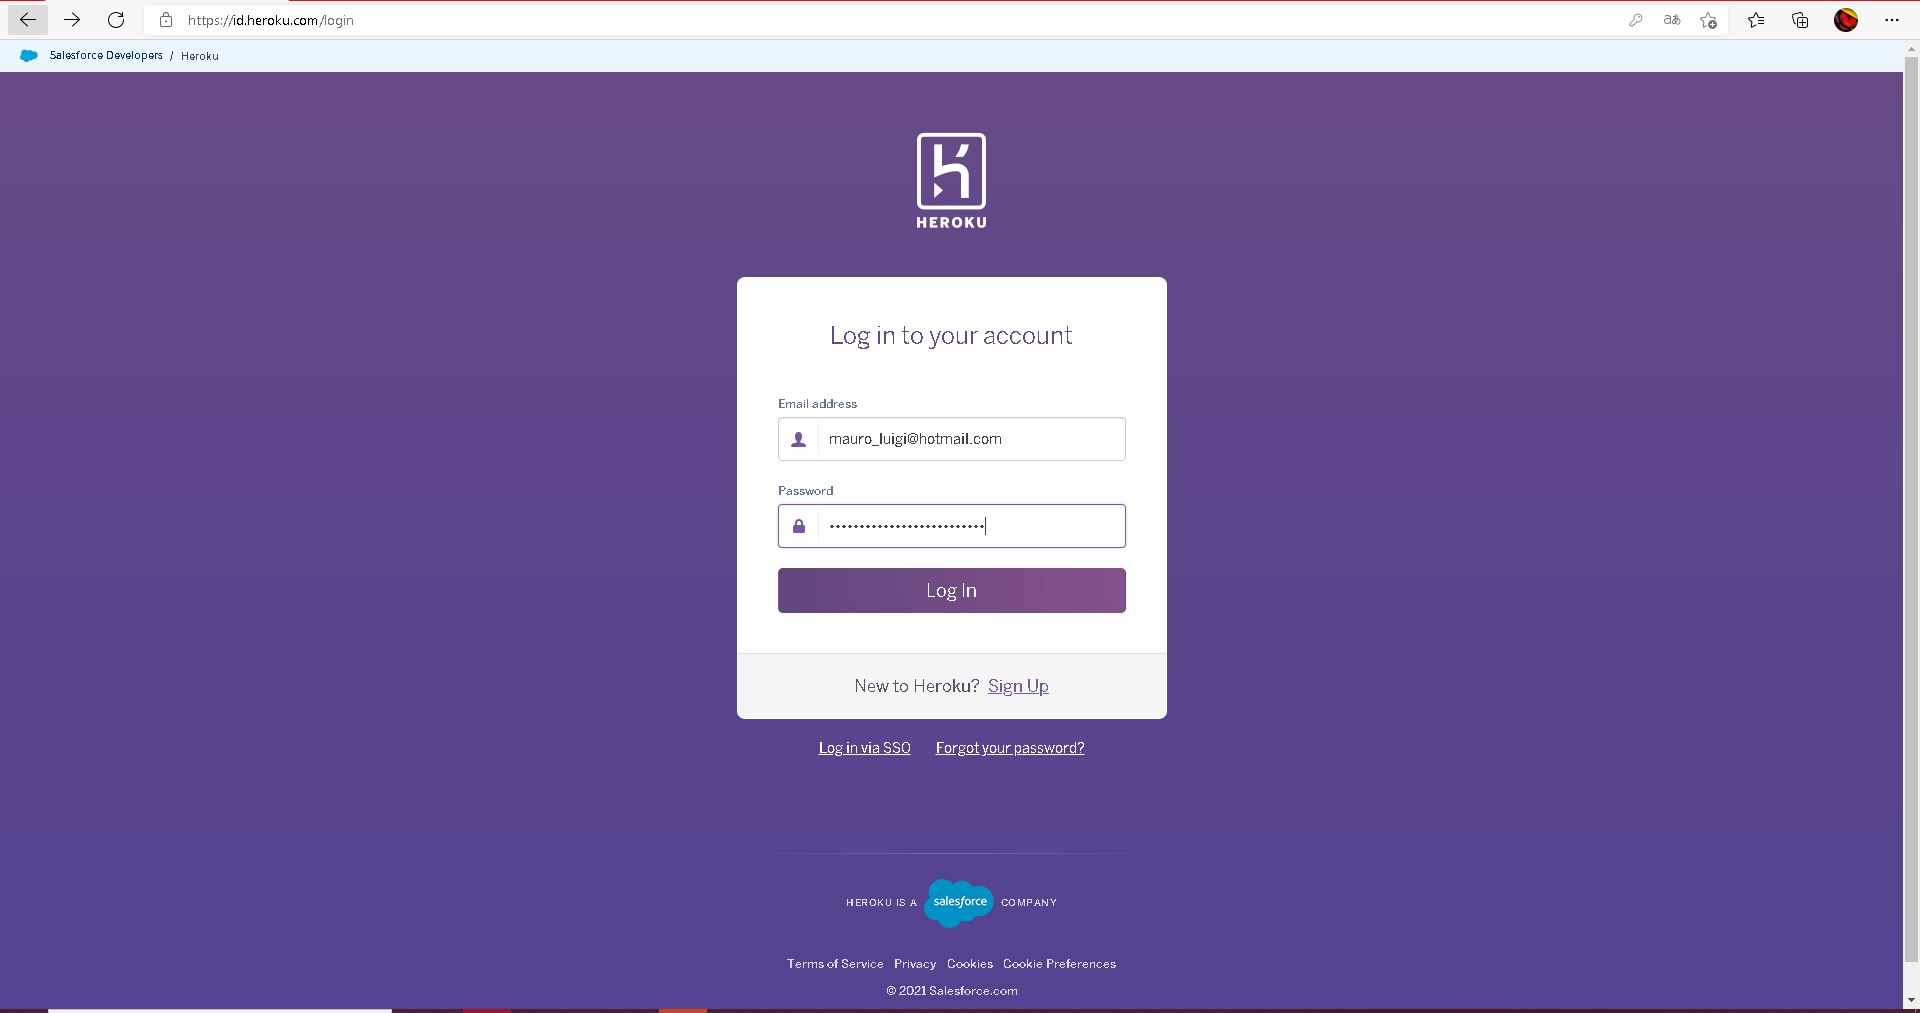
\includegraphics[width=0.8\textwidth]{capturasProyectoBase/resultado5.PNG} \par\vspace{0.5cm}
    \end{figure}
    
    \clearpage
    
    \begin{figure}[h]
        \caption{Ver categoria}
        \centering
        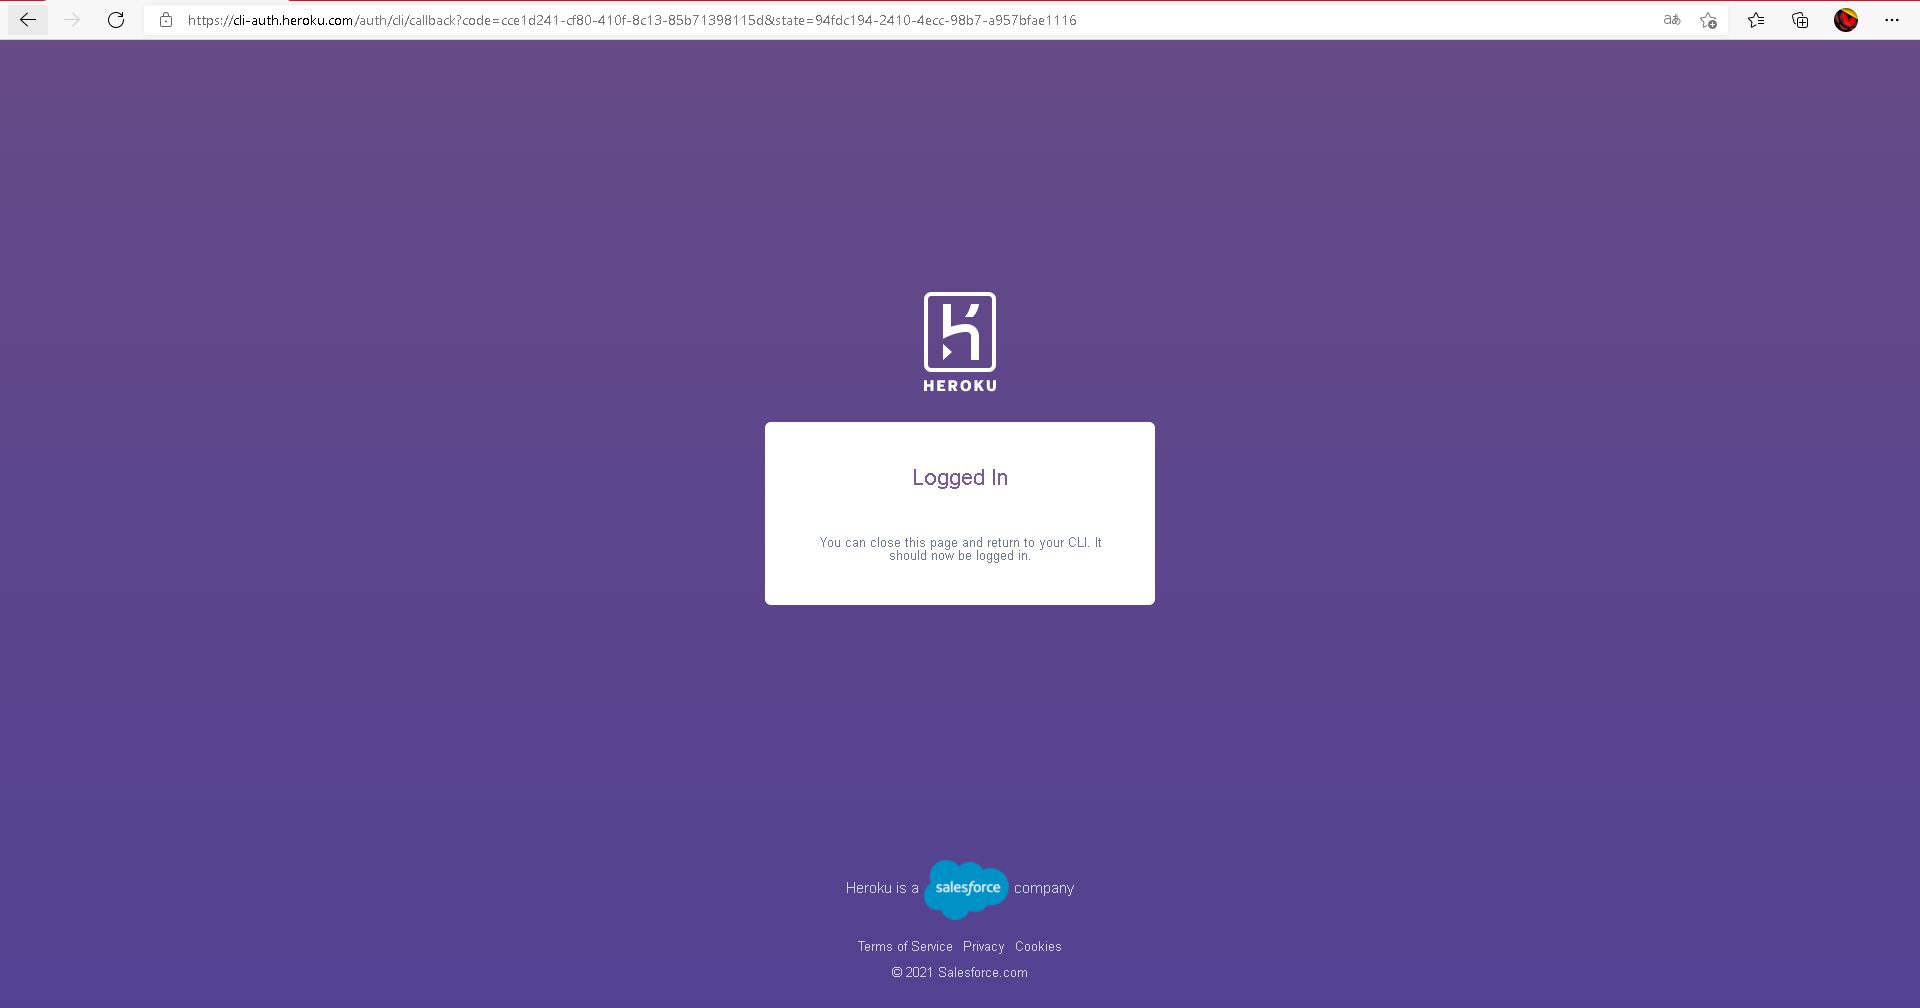
\includegraphics[width=0.8\textwidth]{capturasProyectoBase/resultado6.PNG} \par\vspace{0.5cm}
    \end{figure}
    
    \begin{figure}[h]
        \caption{Crear categoria (formulario)}
        \centering
        \includegraphics[width=0.8\textwidth]{capturasProyectoBase/resultado8.PNG} \par\vspace{0.5cm}
    \end{figure}
    
    \clearpage
    
    \begin{figure}[h]
        \caption{Crear categoria (resultado)}
        \centering
        \includegraphics[width=0.8\textwidth]{capturasProyectoBase/resultado9.PNG} \par\vspace{0.5cm}
    \end{figure}
    
    \begin{figure}[h]
        \caption{Eliminar categoria (resultado)}
        \centering
        \includegraphics[width=0.8\textwidth]{capturasProyectoBase/resultado10.PNG} \par\vspace{0.5cm}
    \end{figure}
    
    \clearpage
    
    \begin{figure}[h]
        \caption{Actualizar categoria (formulario)}
        \centering
        \includegraphics[width=0.8\textwidth]{capturasProyectoBase/resultado11.PNG} \par\vspace{0.5cm}
    \end{figure}
    
    \begin{figure}[h]
        \caption{Actualizar categoria (resultado)}
        \centering
        \includegraphics[width=0.8\textwidth]{capturasProyectoBase/resultado12.PNG} \par\vspace{0.5cm}
    \end{figure}
    
    \clearpage
    \subsection{Productos}
    
    \begin{figure}[h]
        \caption{Mostrar productos}
        \centering
        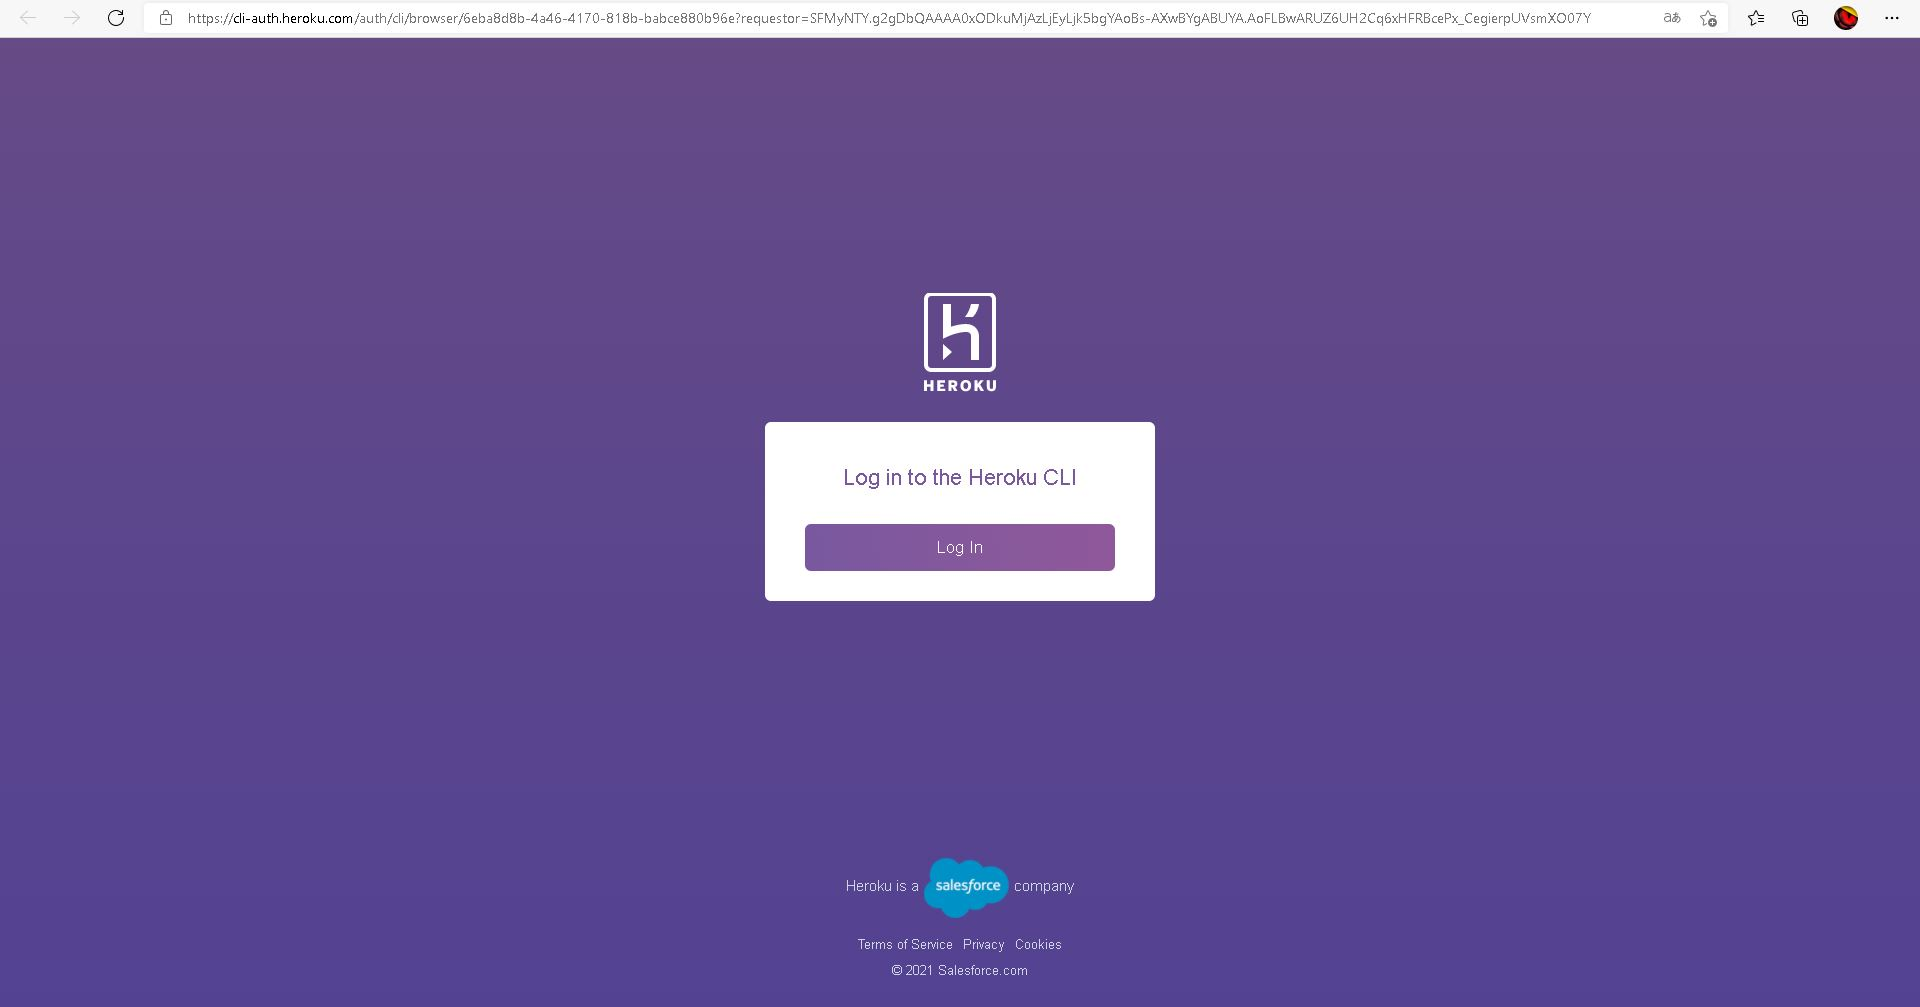
\includegraphics[width=0.8\textwidth]{capturasProyectoBase/resultado4.PNG} \par\vspace{0.5cm}
    \end{figure}
        
    \begin{figure}[h]
        \caption{Ver producto}
        \centering
        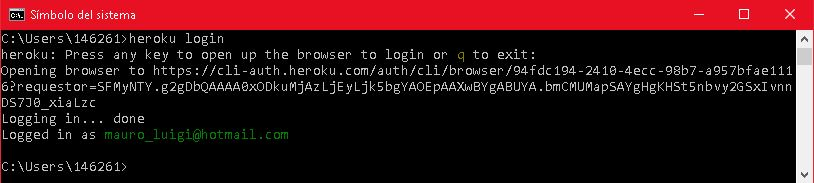
\includegraphics[width=0.8\textwidth]{capturasProyectoBase/resultado7.PNG} \par\vspace{0.5cm}
    \end{figure}
    
    \clearpage
    
    \begin{figure}[h]
        \caption{Crear producto (formulario)}
        \centering
        \includegraphics[width=0.8\textwidth]{capturasProyectoBase/resultado13.PNG} \par\vspace{0.5cm}
    \end{figure}
    
    \begin{figure}[h]
        \caption{Crear producto (resultado)}
        \centering
        \includegraphics[width=0.8\textwidth]{capturasProyectoBase/resultado14.PNG} \par\vspace{0.5cm}
    \end{figure}
    
    \clearpage
    
    \begin{figure}[h]
        \caption{Actualizar producto (formulario)}
        \centering
        \includegraphics[width=0.8\textwidth]{capturasProyectoBase/resultado15.PNG} \par\vspace{0.5cm}
    \end{figure}
    
    \begin{figure}[h]
        \caption{Actualizar producto (resultado)}
        \centering
        \includegraphics[width=0.8\textwidth]{capturasProyectoBase/resultado16.PNG} \par\vspace{0.5cm}
    \end{figure}
    
    \clearpage
    
    \begin{figure}[h]
        \caption{Eliminar producto (resultado)}
        \centering
        \includegraphics[width=0.8\textwidth]{capturasProyectoBase/resultado17.PNG} \par\vspace{0.5cm}
    \end{figure}

\pagebreak

\section{Conclusiones:}
%#########################################################
\subsection{Guadarrama Ascencio Juan Carlos:}

Para el desarrollo de este proyecto, tuvimos que utilzar los servlets, los cuales nos proporcionan varías ventajas: portabilidad, seguridad y rendimiento.

Además podemos identificar algunas de las características de los servlets:

    \begin{enumerate}
        \item Son independientes del servidor utilizado.
        \item Pueden llamar a otros servlets e incluso a métodos de otros servlets.
        \item Pueden obtener información del cliente.
        \item Pueden actuar como enlace entre el cliente y una o varias bases de datos.
        \item Permiten la generación dinámica de código HTML dentro de una propia pagina HTML.
    \end{enumerate}
    
Otra tecnología reelevante para esta práctica fue el uso del driver JDBC la cual nos permite un veloz acceso a una base de datos (en nuestro caso postgreSQL) desde la web además de reducur notablemente la ejecución de instrucciones SQL.
%#########################################################    
\subsection{Ornelas García Luís Ángel:}

El uso de Servlets es bastante común para el desarrollo de páginas web dinámicas, apoyándose del lenguaje Java. Podemos desarrollar desde un simple Servlet que nos muestre una página web, hasta uno que se conecte a una base de datos. Hay posibilidades infinitas a la hora de crear nuestra aplicación web. \par\vspace{0.5cm}
En esta práctica vimos cómo hacer uso de los Servlets, desde hacer una simple tabla de multiplicar hasta manejar directamente una base de datos a través de la página web generada dinámicamente por el propio Servlet. \par\vspace{0.5cm}
Vimos también el uso del controlador de JDBC para conectarnos a una base de datos, en este caso usamos el gestor de base de datos PostgreSQL. Hay que mencionar que el cambiar de controlador haría que tuviéramos que cambiar los Queries para algunas instrucciones, esto es debido a que todos los gestores tienen su propio estándar.
%#########################################################
\pagebreak
\subsection{Sampayo Hernández Mauro:}

Durante el desarrollo de este proyecto se hizo uso de los Servlets, los cuales son una herramienta bastante útil para el desarrollo de aplicaciones Web al proveernos de herramientas que nos permiten tener un mejor control del lado del servidor al momento de manejar la información recibida por parte del cliente en alguna petición o a la accedida desde un pool de conexiones a una Base de Datos. \par\vspace{0.5cm}
De esta manera es que por medio de esta práctica se logró el aprendizaje de estas herramientas para poder ser implementadas en futuras aplicaciones Web que lleguemos a desarrollar para así tener un manejo más dinámico y portable dentro de los servidores de estas. De igual manera se logró un aprendizaje del gestor de bases de datos PostgreSQL, para poder llevar a cabo un mejor manejo y administración de la información contenida dentro de las bases de datos que sean utilizadas en la aplicación Web.

%#########################################################
\pagebreak

\section{Referencias bibliográficas:}

[1] Java Servlet Technology Overview (s. f.). Oracle.\par\vspace{0.1cm}
\textcolor{blue}{https://www.oracle.com/java/technologies/servlet-technology.html} \par\vspace{0.5cm}

[2] Elorduy, V. T. L. E. D. G. (2017, 10 septiembre). Conectores para clientes. Java a tu alcance. \par\vspace{0.1cm} \textcolor{blue}{https://javaparajavatos.wordpress.com/2017/09/09/conectores-para-clientes/} \par\vspace{0.5cm}

[3] Java SE Technologies - Database. (s. f.). Oracle. \par\vspace{0.1cm} \textcolor{blue}{https://www.oracle.com/java/technologies/javase/javase-tech-database.html} \par\vspace{0.5cm}

\end{document}